% Options for packages loaded elsewhere
% Options for packages loaded elsewhere
\PassOptionsToPackage{unicode}{hyperref}
\PassOptionsToPackage{hyphens}{url}
\PassOptionsToPackage{dvipsnames,svgnames,x11names}{xcolor}
%
\documentclass[
  12pt,
  openany]{book}
\usepackage{xcolor}
\usepackage[top=20mm,left=15mm,right=15mm,bottom=20mm]{geometry}
\usepackage{amsmath,amssymb}
\setcounter{secnumdepth}{5}
\usepackage{iftex}
\ifPDFTeX
  \usepackage[T1]{fontenc}
  \usepackage[utf8]{inputenc}
  \usepackage{textcomp} % provide euro and other symbols
\else % if luatex or xetex
  \usepackage{unicode-math} % this also loads fontspec
  \defaultfontfeatures{Scale=MatchLowercase}
  \defaultfontfeatures[\rmfamily]{Ligatures=TeX,Scale=1}
\fi
\usepackage{lmodern}
\ifPDFTeX\else
  % xetex/luatex font selection
\fi
% Use upquote if available, for straight quotes in verbatim environments
\IfFileExists{upquote.sty}{\usepackage{upquote}}{}
\IfFileExists{microtype.sty}{% use microtype if available
  \usepackage[]{microtype}
  \UseMicrotypeSet[protrusion]{basicmath} % disable protrusion for tt fonts
}{}
\makeatletter
\@ifundefined{KOMAClassName}{% if non-KOMA class
  \IfFileExists{parskip.sty}{%
    \usepackage{parskip}
  }{% else
    \setlength{\parindent}{0pt}
    \setlength{\parskip}{6pt plus 2pt minus 1pt}}
}{% if KOMA class
  \KOMAoptions{parskip=half}}
\makeatother
% Make \paragraph and \subparagraph free-standing
\makeatletter
\ifx\paragraph\undefined\else
  \let\oldparagraph\paragraph
  \renewcommand{\paragraph}{
    \@ifstar
      \xxxParagraphStar
      \xxxParagraphNoStar
  }
  \newcommand{\xxxParagraphStar}[1]{\oldparagraph*{#1}\mbox{}}
  \newcommand{\xxxParagraphNoStar}[1]{\oldparagraph{#1}\mbox{}}
\fi
\ifx\subparagraph\undefined\else
  \let\oldsubparagraph\subparagraph
  \renewcommand{\subparagraph}{
    \@ifstar
      \xxxSubParagraphStar
      \xxxSubParagraphNoStar
  }
  \newcommand{\xxxSubParagraphStar}[1]{\oldsubparagraph*{#1}\mbox{}}
  \newcommand{\xxxSubParagraphNoStar}[1]{\oldsubparagraph{#1}\mbox{}}
\fi
\makeatother


\usepackage{longtable,booktabs,array}
\newcounter{none} % for unnumbered tables
\usepackage{calc} % for calculating minipage widths
% Correct order of tables after \paragraph or \subparagraph
\usepackage{etoolbox}
\makeatletter
\patchcmd\longtable{\par}{\if@noskipsec\mbox{}\fi\par}{}{}
\makeatother
% Allow footnotes in longtable head/foot
\IfFileExists{footnotehyper.sty}{\usepackage{footnotehyper}}{\usepackage{footnote}}
\makesavenoteenv{longtable}
\usepackage{graphicx}
\makeatletter
\newsavebox\pandoc@box
\newcommand*\pandocbounded[1]{% scales image to fit in text height/width
  \sbox\pandoc@box{#1}%
  \Gscale@div\@tempa{\textheight}{\dimexpr\ht\pandoc@box+\dp\pandoc@box\relax}%
  \Gscale@div\@tempb{\linewidth}{\wd\pandoc@box}%
  \ifdim\@tempb\p@<\@tempa\p@\let\@tempa\@tempb\fi% select the smaller of both
  \ifdim\@tempa\p@<\p@\scalebox{\@tempa}{\usebox\pandoc@box}%
  \else\usebox{\pandoc@box}%
  \fi%
}
% Set default figure placement to htbp
\def\fps@figure{htbp}
\makeatother





\setlength{\emergencystretch}{3em} % prevent overfull lines

\providecommand{\tightlist}{%
  \setlength{\itemsep}{0pt}\setlength{\parskip}{0pt}}



 


\usepackage{fancyhdr}
\pagestyle{fancy}
\fancyhead[R]{ENSGSI 2AP - Mécanique des Solidés Déformables}

\fancyfoot[L]{Guillaume PRONOST | Fabio CRUZ}
\fancyfoot[C]{\thepage}
\fancyfoot[R]{ENSGSI - 2023/2024}
\renewcommand{\footrulewidth}{0.3pt}% default is 0pt
\setlength{\headheight}{15pt}
\usepackage{mathtools}
\usepackage[makeroom]{cancel}

\usepackage{fancyhdr} % en-têtes et pieds de page

\let\paragraph\oldparagraph
\let\subparagraph\oldsubparagraph

\usepackage[explicit]{titlesec} % titres de chapitres, sections, etc.




% Mise en forme des titres de chapitres : 

\titlespacing*{\chapter}{0pt}{-50pt}{5pt} 
\titleformat{\chapter}[display]
  {\LARGE\bfseries\sffamily}
  {}
  {12pt}
  {%
\begin{tcolorbox}[
	enhanced jigsaw,
	title={Mécanique du Point Matériel},
	fonttitle=\normalsize\sffamily,
	halign=center,
	top=\baselineskip,
	colback=red!10!white,
	colframe=red!50!black,
	boxrule=1.2pt,
	colbacktitle=red!50!white!75!black,
	attach boxed title to top center={yshift=-0.25mm-\tcboxedtitleheight/			2,yshifttext=2mm-\tcboxedtitleheight/2},
	boxed title style={enhanced,boxrule=0.5mm,
	frame code={ \path[tcb fill frame] ([xshift=-4mm]frame.west) -- 				(frame.north west)
    -- (frame.north east) -- ([xshift=4mm]frame.east)
    -- (frame.south east) -- (frame.south west) -- cycle; },
    interior code={ \path[tcb fill interior] ([xshift=-2mm]interior.west)
    -- (interior.north west) -- (interior.north east)
    -- ([xshift=2mm]interior.east) -- (interior.south east) -- (interior.south 		west)
    -- cycle;}  },
 	drop shadow]
    #1
\end{tcolorbox}
}

\renewcommand\thesection{\arabic{section}}
\makeatletter
\@ifpackageloaded{tcolorbox}{}{\usepackage[skins,breakable]{tcolorbox}}
\@ifpackageloaded{fontawesome5}{}{\usepackage{fontawesome5}}
\definecolor{quarto-callout-color}{HTML}{909090}
\definecolor{quarto-callout-note-color}{HTML}{0758E5}
\definecolor{quarto-callout-important-color}{HTML}{CC1914}
\definecolor{quarto-callout-warning-color}{HTML}{EB9113}
\definecolor{quarto-callout-tip-color}{HTML}{00A047}
\definecolor{quarto-callout-caution-color}{HTML}{FC5300}
\definecolor{quarto-callout-color-frame}{HTML}{acacac}
\definecolor{quarto-callout-note-color-frame}{HTML}{4582ec}
\definecolor{quarto-callout-important-color-frame}{HTML}{d9534f}
\definecolor{quarto-callout-warning-color-frame}{HTML}{f0ad4e}
\definecolor{quarto-callout-tip-color-frame}{HTML}{02b875}
\definecolor{quarto-callout-caution-color-frame}{HTML}{fd7e14}
\makeatother
\makeatletter
\@ifpackageloaded{caption}{}{\usepackage{caption}}
\AtBeginDocument{%
\ifdefined\contentsname
  \renewcommand*\contentsname{Table of contents}
\else
  \newcommand\contentsname{Table of contents}
\fi
\ifdefined\listfigurename
  \renewcommand*\listfigurename{List of Figures}
\else
  \newcommand\listfigurename{List of Figures}
\fi
\ifdefined\listtablename
  \renewcommand*\listtablename{List of Tables}
\else
  \newcommand\listtablename{List of Tables}
\fi
\ifdefined\figurename
  \renewcommand*\figurename{Figure}
\else
  \newcommand\figurename{Figure}
\fi
\ifdefined\tablename
  \renewcommand*\tablename{Table}
\else
  \newcommand\tablename{Table}
\fi
}
\@ifpackageloaded{float}{}{\usepackage{float}}
\floatstyle{ruled}
\@ifundefined{c@chapter}{\newfloat{codelisting}{h}{lop}}{\newfloat{codelisting}{h}{lop}[chapter]}
\floatname{codelisting}{Listing}
\newcommand*\listoflistings{\listof{codelisting}{List of Listings}}
\usepackage{amsthm}
\theoremstyle{plain}
\newtheorem{theorem}{Theorem}[section]
\theoremstyle{remark}
\AtBeginDocument{\renewcommand*{\proofname}{Proof}}
\newtheorem*{remark}{Remark}
\newtheorem*{solution}{Solution}
\newtheorem{refremark}{Remark}[section]
\newtheorem{refsolution}{Solution}[section]
\makeatother
\makeatletter
\makeatother
\makeatletter
\@ifpackageloaded{caption}{}{\usepackage{caption}}
\@ifpackageloaded{subcaption}{}{\usepackage{subcaption}}
\makeatother
\usepackage{bookmark}
\IfFileExists{xurl.sty}{\usepackage{xurl}}{} % add URL line breaks if available
\urlstyle{same}
% fallback for those not using the hyperref driver hyperxmp:
\makeatletter
\@ifundefined{xmpquote}{\newcommand{\xmpquote}[1]{#1}}{}
\makeatother
\hypersetup{
  colorlinks=true,
  linkcolor={Maroon},
  filecolor={Maroon},
  citecolor={Blue},
  urlcolor={Blue},
  pdfcreator={LaTeX via pandoc}}


\author{}
\date{}
\begin{document}
\frontmatter


\mainmatter
\$\$

\newcommand\Ccancel[2][black]{
    \let\OldcancelColor\CancelColor
    \renewcommand\CancelColor{\color{#1}}
    \cancel{#2}
    \renewcommand\CancelColor{\OldcancelColor}
}

\$\$

\chapter{Lecture obligatoire}\label{lecture-obligatoire}

\begin{itemize}
\tightlist
\item
  Chapitre 1 de ..
\end{itemize}

\section{Slides avec des idées
clés}\label{slides-avec-des-iduxe9es-cluxe9s}

\chapter{Qu'est ce que c'est la
Cinématique?}\label{quest-ce-que-cest-la-cinuxe9matique}

La cinématique est une branche de la mécanique qui exprime sous forme
mathématique le mouvement des corps. La cinématique du point constitue
l'étude du mouvement d'un point indépendamment des causes qui ont
engendré ce mouvement.

\begin{tcolorbox}[enhanced jigsaw, arc=.35mm, bottomrule=.15mm, bottomtitle=1mm, breakable, colback=white, colbacktitle=quarto-callout-note-color!10!white, colframe=quarto-callout-note-color-frame, coltitle=black, left=2mm, leftrule=.75mm, opacityback=0, opacitybacktitle=0.6, rightrule=.15mm, title=\textcolor{quarto-callout-note-color}{\faInfo}\hspace{0.5em}{Point matériel}, titlerule=0mm, toprule=.15mm, toptitle=1mm]

Il arrive souvent que l'on puisse décrire et prédire le mouvement d'un
objet par les lois de la dynamique, en associant l'objet à un unique
point géométrique auquel on attribue la masse \(m\) de l'objet. C'est ce
qu'on appelle un \emph{point matériel}.

Ce point matériel constitue un \emph{modèle} de l'objet étudié. Il
s'agit donc d'une approximation permettant une application simple de
lois physiques sur cet objet. La modélisation du comportement de l'objet
sous la forme d'un point matériel constitue une approximation de son
comportement réel.

\end{tcolorbox}

\chapter{Rappels sur les vecteurs et les espaces
vectoriels}\label{rappels-sur-les-vecteurs-et-les-espaces-vectoriels}

\section{Comparaison des vecteurs}\label{comparaison-des-vecteurs}

Deux vecteurs non nuls \(\va u\) et \(\va v\) sont
\textbf{\emph{colinéaires}} si et seulement si il existe un nombre réel
\(k\) tel que \(\va v = k*\va u\). Autrement dit, deux vecteurs sont
colinéaires si l'un est un multiple de l'autre.

Le \textbf{\emph{produit scalaire}} de deux vecteurs \(\va u\) et
\(\va v\) peut être défini comme:

\[
\newcommand\mcy{{\mathcal{y}}}
\va u .\va v = \left|\left|\va u\right|\right| \left|\left|\va v\right|\right| \cos{\theta}
\]

où \(\theta\) est l'angle formé entre \(\va u\) et \(\va v\)

Deux vecteurs non nuls \(\va u\) et \(\va v\) sont
\emph{\textbf{orthogonaux}} si et seulement si leur produit scalaire est
nul : \(\va u .\va v = 0\)

\section{Base d'un espace vectoriel}\label{base-dun-espace-vectoriel}

Soit \(E\) un espace vectoriel.

Une famille de vecteurs \(F\) = (\(\va i_1\), \(\va i_2\), \ldots{}
\(\va i_n\)) de \(E\) est dite \emph{libre} et ses vecteurs sont dit
liénairements indépendants, lorsque

\begin{align*}

\forall \ \lambda_1,\ \lambda_2,\ ...,\ \lambda_n \in E,\ \lambda_1 \va i_1 + \lambda_2 \va i_2 + ... + \lambda_n \va i_n = \va 0 \implies \lambda_1= \lambda_2= ...=\lambda_n = 0

\end{align*}

Une famille qui n'est pas libre est dite \emph{liée}.

Une famille de vecteurs \(F\) = (\(\va i_1\), \(\va i_2\), \ldots{}
\(\va i_n\)) de \(E\) est dite \emph{génératrice} lorsque tout vecteur
\(\va v \in E\) est combinaison des vecteurs de \(F\).

Une famille de vecteurs \(F\) = (\(\va i_1\), \(\va i_2\), \ldots{}
\(\va i_n\)) de \(E\) est dite \textbf{\emph{base}} de \(E\) lorsque
qu'elle est libre et génératrice.

\chapter{Repère}\label{repuxe8re}

Soit \(E\) un espace vectoriel de dimension \(n\), \(A\) un espace
affine sur \(E\). Soit (\(\va i_1\), \(\va i_2\), \ldots{} \(\va i_n\))
une base de \(E\) et \(M\) un point de l'espace affine \(A\). Alors
l'ensemble (\(A\), \(\va i_1\), \(\va i_2\), \ldots{} \(\va i_n\))
constitue un \textbf{\emph{repère}} de \(E\).

\section{Repère orthonormé direct en dimension 2 et
3}\label{repuxe8re-orthonormuxe9-direct-en-dimension-2-et-3}

Dans ce chapitre et les suivants, on s'interessera uniquement à des
espaces de dimension 2 (problème plan) et de dimension 3 (problème en
3D). Dans ce contexte, les différents repères utilisés seront toujours
des repères orthonormés directs.

Un repère (\(A\), \(\va i_1\), \ldots{} \(\va i_n\)) est dit
\textbf{\emph{orthonormé}} si tout les vecteurs (\(\va i_1\), \ldots{}
\(\va i_n\)) composant ce repère sont des vecteurs
\textbf{\emph{unitaires}}, c'est-à-dire qu'ils sont de norme 1 :

\begin{align*}
 \left|\left|\va i_1\right|\right|= ... =\left|\left|\va i_n\right|\right|= 1
\end{align*}

Un repère (\(A\), \(\va i_1\), \ldots{} \(\va i_n\)) de dimension 2 ou 3
est dit \textbf{\emph{direct}} si il respecte la règle dite du
``bonhomme d'Ampère'' ou de la ``main droite''. Dans le cas contraire,
le repère est dit \textbf{\emph{indirect}}.

\section{Repérage d'un point
matériel}\label{repuxe9rage-dun-point-matuxe9riel}

\section{Référentiel}\label{ruxe9fuxe9rentiel}

Pour commence à discuter du mouvement d'un corps ou d'un point, il est
nécessaire de définir par rapport à quoi le mouvement sera mesuré.

Un \textbf{\emph{référentiel}} est un solide servant de référence pour
décrire le mouvement des objets. Les vitesses et accélérations sont
définies par rapport à ce référentiel.

Sauf indication contraire, nous utiliserons le référentiel terrestre.

Exemples de référentiels :

\begin{itemize}
\tightlist
\item
  Le référentiel héliocentrique (ou référentiel de Kepler)
\item
  Le référentiel géocentrique
\item
  Le référentiel terrestre
\end{itemize}

Nous supposerons qu'il existe un temps absolu : deux observateurs en
mouvement relatifs peuvent attribuer les mêmes dates aux mêmes
événements.

\section{Trajectoire d'un point}\label{trajectoire-dun-point}

On appelle \textbf{\emph{trajectoire}} d'un point, dans un référentiel,
l'ensemble des positions successives occupées par ce point au cours du
temps.

Soit \(O\) un point particulier du référentiel et \(M\) la position du
point matériel. La fonction \(\overrightarrow{OM}(t)\) donne la position
du point matériel \(M\) au cours du temps \(t\). On la nomme
\textbf{\emph{équation horaire}}.

Déterminer cette fonction \(\overrightarrow{OM}(t)\) représente
l'objectif principal de la mécanique du point.

\section{Position d'un point en 2
dimensions}\label{position-dun-point-en-2-dimensions}

On place un observateur à un point \(O\) du référentiel, nommé
\textbf{origine}. On cherche à exprimer la position d'un point matériel
\(M\) par rapport à un repère orthonormé direct (\(O\), \(\va u_1\),
\(\va u_2\)).

\subsection{Coordonnées
cartésiennes}\label{coordonnuxe9es-cartuxe9siennes}

\pandocbounded{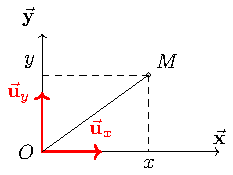
\includegraphics[keepaspectratio]{01-cinematique_files/figure-pdf/unnamed-chunk-1-1.pdf}}

Le point \(M\) est repéré par les coordonnées cartésiennes (\(x\),
\(y\))

\begin{align*}
 \va{OM} &= x \va u_x + y \va u_y \\ x, y \ &\in \ ]-\infty, +\infty[
\end{align*}

Le repère associé aux coordonnées cartésiennes permet de décrire les
coordonnées d'un point \(M(x, y)\) et les composantes d'un vecteur
\(\va V(V_x, V_y)\) sur la base (\(\va u_x\),
\(\va u_y\)).\textbackslash{}

Dans la suite, le référentiel \(R_c\) associé aux coordonnées
cartésiennes sera considéré comme fixe.

Il se peut que les coordonnées cartésiennes ne soient pas les plus
commodes pour décrire la position d'un point matériel. C'est notamment
le cas lorsqu'on veut décrire un mouvement de rotation, tel qu'un
mouvement sur une sphère ou un cylindre.

\subsection{Coordonnées polaires}\label{coordonnuxe9es-polaires}

\pandocbounded{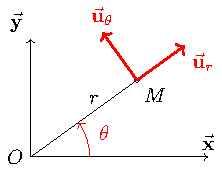
\includegraphics[keepaspectratio]{01-cinematique_files/figure-pdf/unnamed-chunk-2-1.pdf}}

Le point \(M\) est repéré par les coordonnées polaires (\(r\),
\(\theta\)) \begin{align*}
\va{OM} &= r \va u_r  \\ r \ &\in \ [0, +\infty[ \\ \theta \ &\in \ [0, 2\pi[
\end{align*}

Le repère associé aux coordonnées polaires permet de décrire les
coordonnées d'un point \(M ( r, \theta)\) et les composantes d'un
vecteur \(\va V(V_r, V_\theta)\) sur la base (\(\va u_r\),
\(\va u_\theta\)).

Il est important de remarquer que la base dépend de la coordonnée
\(\theta\) du point \(M\).

En général, les coordonnées cartésiennes sont associées au référentiel
terrestre, considéré comme \textbf{\emph{galiléen}}. Les coordonnées
polaires, quant à elles, sont particulièrement adaptées à l'étude des
mouvements de rotation. La base est souvent appelée \textbf{\emph{base
mobile}}. On dit qu'elle est associée au référentiel tournant \(R_T\).

\begin{theorem}[Changement de
base]\protect\hypertarget{thm-base}{}\label{thm-base}

On s'interesse à une base fixe (\(\va u_x\), \(\va u_y\)) et à une base
mobile (\(\va u_r\), \(\va u_\theta\)). Tout les vecteurs des bases sont
unitaires. On a donc :

\begin{align*}

\left|\left|\va u_x\right|\right|=\left|\left|\va u_y\right|\right|=\left|\left|\va u_r\right|\right|=\left|\left|\va u_\theta\right|\right|=1

\end{align*}

\begin{align*}
\va u_r &= \va u_{r_x} + \va u_{r_y} \\
\va u_r &= \cos{\theta}\va u_x + \sin{\theta}\va u_y\\
&\\
\va u_\theta &= \va u_{\theta_x} + \va u_{\theta_y} \\
\va u_\theta &= -\sin{\theta}\va u_x + \cos{\theta}\va u_y
\end{align*}

\pandocbounded{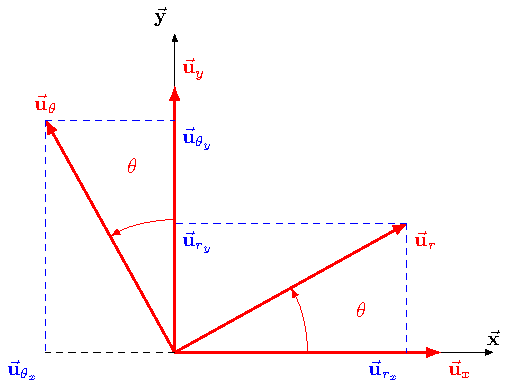
\includegraphics[keepaspectratio]{01-cinematique_files/figure-pdf/unnamed-chunk-3-1.pdf}}

\begin{align*}
\va u_x &= \va u_{x_r} + \va u_{x_\theta} \\
\va u_x &= \cos{\theta}\va u_r - \sin{\theta}\va u_\theta\\
&\\
\va u_y &= \va u_{y_r} + \va u_{y_\theta} \\
\va u_y &= \sin{\theta}\va u_r + \cos{\theta}\va u_\theta
\end{align*}

\pandocbounded{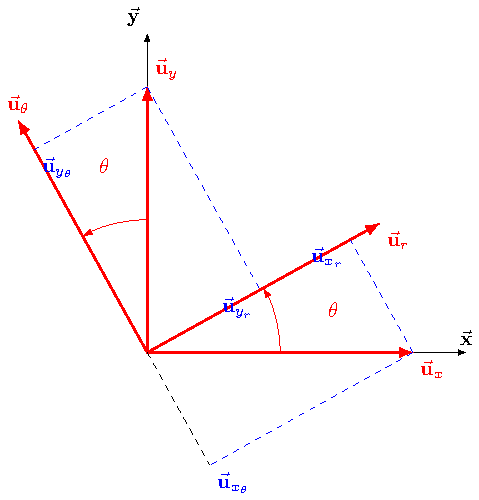
\includegraphics[keepaspectratio]{01-cinematique_files/figure-pdf/unnamed-chunk-4-1.pdf}}

\end{theorem}

On a pu voir que différents systèmes de coordonnées permettaient de
représenter la position du point \(M\). Ainsi :

\begin{align*}
 \overrightarrow{OM} &= x \va u_x + y \va u_y \\ 
 & \text{et}\\
\overrightarrow{OM} &= r \va u_r
\end{align*}

A partir des formules de projections déterminées précedemment, il est
possible d'exprimer les coordonnées cartésiennes (\(x\), \(y\)) en
fonction des coordonnées polaires (\(r\), \(\theta\)) et inversemment.
Ainsi :

\begin{equation*}
    \begin{cases}
      x &= \ r \cos{\theta}  \\
      y &= \ r \sin{\theta} 
    \end{cases}       
\end{equation*}

\chapter{Position d'un point en 3
dimensions}\label{position-dun-point-en-3-dimensions}

On place un observateur à un point \(O\) du référentiel, nommé
\textbf{\emph{origine}}. On cherche à exprimer la position d'un point
matériel \(M\) par rapport à un repère orthonormé direct (\(O\),
\(\va u_1\), \(\va u_2\), \(\va u_3\)).

\subsection{Coordonnées
cartésiennes}\label{coordonnuxe9es-cartuxe9siennes-1}

\pandocbounded{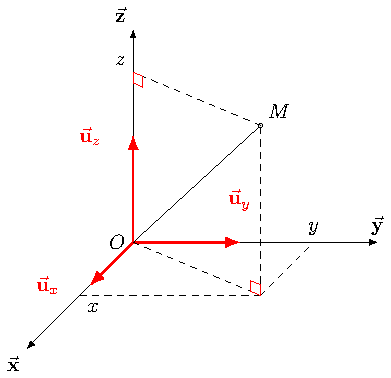
\includegraphics[keepaspectratio]{01-cinematique_files/figure-pdf/unnamed-chunk-5-1.pdf}}

Le point \(M\) est repéré par les coordonnées cartésiennes (\(x\),
\(y\), \(z\)) \begin{align*}
&\va{OM} = x \va u_x + y \va u_y + z \va u_z \\ &x, y, z \ \in \ ]-\infty, +\infty[
\end{align*}

Le repère associé aux coordonnées cartésiennes permet de décrire les
coordonnées d'un point \(M(x, y, z)\) et les composantes d'un vecteur
\(\va V(V_x, V_y, V_z)\) sur la base (\(\va u_x\), \(\va u_y\),
\(\va u_z\)).\textbackslash{}

Dans la suite, le référentiel \(R_c\) associé aux coordonnées
cartésiennes sera considéré comme fixe.

Il se peut que les coordonnées cartésiennes ne soient pas les plus
commodes pour décrire la position d'un point matériel. C'est notamment
le cas lorsqu'on veut décrire un mouvement de rotation, tel qu'un
mouvement sur une sphère ou un cylindre.

\section{Coordonnées cylindriques}\label{coordonnuxe9es-cylindriques}

Ici figure de Coordones cyclindriques

Le point \(M\) est repéré par les coordonnées cylindriques (\(r\),
\(\theta\), \(z\))

\begin{align*}
  \va{OM} &= r \va u_r  \\ r \ &\in \ [0, +\infty[ \\ \theta \ &\in \ [0, 2\pi[ \\ z \ &\in \ ]-\infty, +\infty[
\end{align*}

On utilisera les coordonnées cylindriques dès que la distance à l'axe
\(O_z\) joue un rôle important dans l'exercice.

\subsection{Changement de système de
coordonnées}\label{changement-de-systuxe8me-de-coordonnuxe9es}

A partir des formules de projections déterminées précedemment, il est
possible d'exprimer les coordonnées cartésiennes (\(x\), \(y\), \(z\))
en fonction des coordonnées cylindriques (\(r\), \(\theta\), \(z\)) et
inversemment. Ainsi :

\begin{equation*}
    \begin{cases}
      x &= \ r \cos{\theta}  \\
      y &= \ r \sin{\theta} \\
      z &= \ z
    \end{cases}       
\end{equation*}

\section{Coordonnées sphériques}\label{coordonnuxe9es-sphuxe9riques}

Figure coordones Spériques

On utilisera les coordonnées sphériques dès que la distance \(r\) au
centre O joue un rôle important dans l'exercice.\textbackslash{}

\subsection{Changement de système de
coordonnées}\label{changement-de-systuxe8me-de-coordonnuxe9es-1}

A partir des formules de projections déterminées précedemment, il est
possible d'exprimer les coordonnées cartésiennes (\(x\), \(y\), \(z\))
en fonction des coordonnées sphériques (\(r\), \(\theta\), \(\phi\)) et
inversemment. Ainsi : \begin{equation*}
    \begin{cases}
      x &= \ r \sin{\theta}\cos{\phi}  \\
      y &= \ r \sin{\theta}\sin{\phi} \\
      z &= \ r \cos{\theta}
    \end{cases}       
\end{equation*}

\chapter{Vitesse d'un point}\label{vitesse-dun-point}

En cinématique, la vitesse peut être définie comme est une grandeur qui
mesure pour un mouvement, le rapport de la distance parcourue au temps
écoulé.

Soit \(M\) la position d'un mobile à un instant \(t\). Soit \(R\) un
référentiel et \(O\) un point fixe de ce référentiel. On note
\(\va v(M_{/R})\) le vecteur vitesse du mobile par rapport au
référentiel \(R\).

On peut exprimer alors cette vitesse :

\begin{align*}
 \va v(M_{/R})=\left(\dfrac{d(\va{OM})}{dt}\right)_{/R}
\end{align*}

Sauf mention contraire le référentiel \(R_c\) par rapport auquel nous
calculerons la vitesse sera celui associé aux coordonnées cartésiennes.
Dans ce référentiel \(R_c\), l'origine \(O\) ainsi que la base
(\(\va u_x\), \(\va u_y\), \(\va u_z\)) sont fixes.

\section{Expression de la vitesse en coordonnées
cartésiennes}\label{expression-de-la-vitesse-en-coordonnuxe9es-cartuxe9siennes}

Soit (\(\va u_x\), \(\va u_y\), \(\va u_z\)) la base des coordonnées
cartésiennes.

\begin{align*}
    &\va v(M_{/R_c})=\left(\frac{d(\va{OM})}{dt}\right)_{/Rc} \ \ \text{avec} \ \ \va{OM} = x \va u_x + y \va u_y + z \va u_z\\
    &\va v(M_{/R_c})=\left(\frac{d(x \va u_x + y \va u_y + z \va u_z)}{dt}\right)_{/R}\\
    &\va v(M_{/R_c})=\frac{dx}{dt}\va u_x + 
    \let\OldcancelColor\CancelColor
    \renewcommand\CancelColor{\color{red}}
    \cancel{x\left(\frac{d(\va u_x)}{dt}\right)_{/R_c}}
    \renewcommand\CancelColor{\OldcancelColor}
 + \frac{dy}{dt}\va u_y + 
    \let\OldcancelColor\CancelColor
    \renewcommand\CancelColor{\color{red}}
    \cancel{y\left(\frac{d(\va u_y)}{dt}\right)_{/R_c}}
    \renewcommand\CancelColor{\OldcancelColor}
 + \frac{dz}{dt}\va u_z +  
    \let\OldcancelColor\CancelColor
    \renewcommand\CancelColor{\color{red}}
    \cancel{z\left(\frac{d(\va u_z)}{dt}\right)_{/R_c}}
    \renewcommand\CancelColor{\OldcancelColor}
\\


    \va v(M_{/R_c})=\dfrac{dx}{dt}\va u_x + \dfrac{dy}{dt}\va u_y + \dfrac{dz}{dt}\va u_z \\
\end{align*}

Les vecteurs \(\va u_x\), \(\va u_y\), et \(\va u_z\) et sont
\textbf{constants} dans \(R_c\) , donc leur dérivée est \textbf{nulle}.

\section{Expression de la vitesse en coordonnées
polaires}\label{expression-de-la-vitesse-en-coordonnuxe9es-polaires}

La vitesse est ici calculée par rapport au référentiel associé aux
coordonnées cartésiennes. Elle s'exprime sur la base des coordonnées
polaires (\(\va u_r\), \(\va u_\theta\)).

\begin{align*}
    &\va v(M_{/R_c})=\left(\frac{d(\va{OM})}{dt}\right)_{/Rc} \ \ \text{avec} \ \ \va{OM} = r \va u_r\\
    &\va v(M_{/R_c})=\left(\frac{d(r \va u_r)}{dt}\right)_{/R}\\
    &\va v(M_{/R_c})=\frac{dr}{dt}\va u_r + r\left(\frac{d(\va u_r)}{dt}\right)_{/R_c} 
\end{align*}

Figure ici

\textbf{Problème :} le vecteur \(\va u_r\) n'est \textbf{pas constant}
dans \(R_c\), donc sa dérivée n'est \textbf{pas nulle}.

\begin{theorem}[Dérivation des vecteurs de la base mobile (\(\va u_r\),
\(\va u_\theta\))]\protect\hypertarget{thm-derivation}{}\label{thm-derivation}

\begin{align*}
  \left(\frac{d(\va u_r)}{dt}\right)_{/Rc} &= \frac{d\theta}{dt}\va u_\theta\\
  \left(\frac{d(\va u_\theta)}{dt}\right)_{/Rc} &= -\frac{d\theta}{dt}\va u_r
\end{align*}

\textbf{A connaître !}

\end{theorem}

Si on applique ces expressions dans le calcul précédent, on obtient
finalement : \begin{align*}
    &\va v(M_{/R_c})=\frac{dr}{dt}\va u_r + r\left(\frac{d(\va u_r)}{dt}\right)_{/R_c}\\
    &\tikz[baseline]{
            \node[fill=red!20,anchor=base,rounded corners]
            {$\va v(M_{/R_c})=\dfrac{dr}{dt}\va u_r + r\dfrac{d\theta}{dt}\va u_\theta$};
        } 
\end{align*}

\subsection{Remarques sur la notation}\label{remarques-sur-la-notation}

On écrit \(\dfrac{dr}{dt}\) et \(\dfrac{d\theta}{dt}\) sans préciser le
référentiel par rapport auquel on dérive car \(r\) est défini par
rapport à l'origine \(O\), commune au repère cartésien et polaire, et
\(\theta\) est défini par rapport à l'axe \(\va x\) qui est fixe.

Les valeurs de \(r(t)\) et \(\theta(t)\) \textbf{\emph{ne dépendent pas
du référentiel}}.

On écrit \(\left(\dfrac{d(\va u_r)}{dt}\right)_{/R_c}\) et
\(\left(\dfrac{d(\va u_\theta)}{dt}\right)_{/R_c}\) en précisant le
référentiel par rapport auquel on dérive car l'expression de ces
vecteurs dépend du référentiel.

Dans le référentiel cartésien \(R_c\), les composantes de \(\va u_r\) et
\(\va u_\theta\) sur (\(\va u_x\), \(\va u_y\)) sont (\(\cos{\theta}\),
\(\sin{\theta}\)) et (\(-\sin{\theta}\), \(\cos{\theta}\)). Comme
\(\theta\) dépend généralement du temps, la dérivée de ces composantes
par rapport à \(R_c\) n'est pas nulle.

Dans le référentiel tournant \(R_T\), les composantes de \(\va u_r\) et
\(\va u_\theta\) sur (\(\va u_r\), \(\va u_\theta\)) sont (\(1\), \(0\))
et (\(0\), \(1\)).

La dérivée par rapport à \(R_T\) est nulle. Ainsi, la dérivation de ces
vecteurs aura un résultat différent selon le référentiel de dérivation
choisi. Elle \textbf{\emph{dépend du référentiel}}.

\section{Expression de la vitesse en coordonnées
cylindriques}\label{expression-de-la-vitesse-en-coordonnuxe9es-cylindriques}

La vitesse est ici calculée par rapport au référentiel associé aux
coordonnées cartésiennes. Elle s'exprime sur la base des coordonnées
cylindriques (\(\va u_r\), \(\va u_\theta\), \(\va u_z\)).

\begin{flalign*}
    &\va v(M_{/R_c})=\left(\frac{d(\va{OM})}{dt}\right)_{/Rc} \ \ \text{avec} \ \ \va{OM} = r \va u_r + z \va u_z&\\
    &\va v(M_{/R_c})=\left(\frac{d(r \va u_r + z \va u_z)}{dt}\right)_{/R}\\
    &\va v(M_{/R_c})=\frac{dr}{dt}\va u_r + r\left(\frac{d(\va u_r)}{dt}\right)_{/R_c} + \frac{dz}{dt}\va u_z +  
    \let\OldcancelColor\CancelColor
    \renewcommand\CancelColor{\color{red}}
    \cancel{z\left(\frac{d(\va u_z)}{dt}\right)_{/R_c}}
    \renewcommand\CancelColor{\OldcancelColor}
\\
    &\tikz[baseline]{
            \node[fill=red!20,anchor=base,rounded corners]
            {$\va v(M_{/R_c})=\dfrac{dr}{dt}\va u_r + r\dfrac{d\theta}{dt}\va u_\theta + \dfrac{dz}{dt}\va u_z$};
        }  
\end{flalign*}

Figure ici

\section{Expression de la vitesse en coordonnées
sphériques}\label{expression-de-la-vitesse-en-coordonnuxe9es-sphuxe9riques}

La vitesse est ici calculée par rapport au référentiel associé aux
coordonnées cartésiennes. Elle s'exprime sur la base des coordonnées
sphériques (\(\va u_r\), \(\va u_\theta\), \(\va u_\phi\)).

\begin{flalign*}
    &\va v(M_{/R_c})=\left(\frac{d(\va{OM})}{dt}\right)_{/Rc} \ \ \text{avec} \ \ \va{OM} = r \va u_r&\\
    &\va v(M_{/R_c})=\left(\frac{d(r \va u_r)}{dt}\right)_{/R}\\
    &\va v(M_{/R_c})=\frac{dr}{dt}\va u_r + r\left(\frac{d(\va u_r)}{dt}\right)_{/R_c}\\
    &\tikz[baseline]{
            \node[fill=red!20,anchor=base,rounded corners]
            {$\va v(M_{/R_c})=\dfrac{dr}{dt}\va u_r + r\dfrac{d\theta}{dt}\va u_\theta + r\sin{\theta}\dfrac{d\phi}{dt}\va u_\phi$};
        }  
\end{flalign*}

Figure ici

\chapter{Accélération d'un point}\label{accuxe9luxe9ration-dun-point}

En cinématique, l'accélération peut être définie comme est une grandeur
qui mesure pour un mouvement, le rapport de la variation de vitesse de
l'objet en fonction du temps.

Soit \(M\) la position d'un mobile à un instant \(t\). Soit \(R\) un
référentiel et \(O\) un point fixe de ce référentiel.\textbackslash{} On
note \(\va \gamma(M_{/R})\) le vecteur accélération du mobile par
rapport au référentiel \(R\).\textbackslash{} On peut exprimer alors
cette accélération :

\begin{align*}
    &\va \gamma(M_{/R})=\left(\frac{d(\va v(M_{/R}))}{dt}\right)_{/R}\\
    &\tikz[baseline]{
        \node[fill=red!20,anchor=base,rounded corners]
        {$\va \gamma(M_{/R})=\left(\dfrac{d^2(\va{OM})}{dt^2}\right)_{/R}$};
    } 
\end{align*}

Comme dans le cas de la vitesse, le référentiel par rapport auquel nous
calculerons l'accélération sera, sauf mention contraire, celui associé
aux coordonnées cartésiennes. Dans ce référentiel \(R_c\), l'origine
\(O\) ainsi que la base (\(\va u_x\), \(\va u_y\), \(\va u_z\)) sont
fixes.

\section{Expression de l'accélération en coordonnées
cartésiennes}\label{expression-de-laccuxe9luxe9ration-en-coordonnuxe9es-cartuxe9siennes}

Soit (\(\va u_x\), \(\va u_y\), \(\va u_z\)) la base des coordonnées
cartésiennes.

\begin{tcolorbox}[enhanced jigsaw, arc=.35mm, bottomrule=.15mm, bottomtitle=1mm, breakable, colback=white, colbacktitle=quarto-callout-tip-color!10!white, colframe=quarto-callout-tip-color-frame, coltitle=black, left=2mm, leftrule=.75mm, opacityback=0, opacitybacktitle=0.6, rightrule=.15mm, title=\textcolor{quarto-callout-tip-color}{\faLightbulb}\hspace{0.5em}{Tip}, titlerule=0mm, toprule=.15mm, toptitle=1mm]

\begin{align*}

&\va \gamma(M_{/R_c})=\left(\frac{d^2(\va{OM})}{dt^2}\right)_{/R_c} \ \ \text{avec} \ \ \va{OM} = x \va u_x + y \va u_y + z \va u_z\\
\va \gamma(M_{/R_c})=\dfrac{d^2x}{dt^2}\va u_x + \dfrac{d^2y}{dt^2}\va u_y + \dfrac{d^2z}{dt^2}\va u_z

\end{align*}

\end{tcolorbox}

On applique la même méthode de calcul que pour la vitesse.

\section{Expression de l'accélération en coordonnées
polaires}\label{expression-de-laccuxe9luxe9ration-en-coordonnuxe9es-polaires}

L'accélération est ici calculée par rapport au référentiel associé aux
coordonnées cartésiennes. Elle s'exprime sur la base des coordonnées
polaires (\(\va u_r\), \(\va u_\theta\)).

\section{Expression de l'accélération en coordonnées
cylindriques}\label{expression-de-laccuxe9luxe9ration-en-coordonnuxe9es-cylindriques}

L'accélération est ici calculée par rapport au référentiel associé aux
coordonnées cartésiennes. Elle s'exprime sur la base des coordonnées
cylindriques (\(\va u_r\), \(\va u_\theta\), \(\va u_z\)).

Figure ici


\backmatter


\end{document}
